\documentclass[psamsfonts]{amsart}

%-------Packages---------
\usepackage{amsmath,amssymb,amsthm}
\usepackage{graphicx}
\usepackage{pdfpages}

\usepackage[all,arc]{xy}
\usepackage{mathrsfs}
\usepackage{bbm}
\usepackage[margin=1.0in]{geometry}

\usepackage{svg}
\usepackage{pdfpages}
\usepackage{verbatimbox}
\usepackage{xcolor}
\usepackage{adjustbox}
\definecolor{shadecolor}{rgb}{0.94, 0.94, 0.94}
\setlength\parindent{0pt}


\setlength{\voffset}{-0.50in}
%\setlength{\headsep}{10pt}

\title{ORIE 4741: Project Midterm Report}
\author{David Lee (dyl44), Clara Ong Lishan (lo88), Zilong Wang (zw243)}
\date{October 27, 2016}

\begin{document}
\maketitle

\underline{NOTE}: Our project topic is based on the INFORMS competition. Much of the information was only just released by the organizers. Therefore, most of our time was spent on trying to understand the data. There are some parts of the data which we still do not understand, and we are waiting for the organizer's clarification. 

\subsection*{Abstract}
\hfill \\

In order for a crop variety to become commercialised, it often has to undergo several rounds of strict testing and experimentation to ensure that it offers good yield. Throughout these multiple phases of testing, crop varieties are often benchmarked against their ``peers" and successfully commercialised varieties that came before by their yield. Every year, varieties that fail to make the cut are discontinued, while those that survive compete again in the following year with newly introduced varieties.\\
\\
 The primary goal of the INFORMS competition is that given past data, we should develop a prediction model that can be used to predict the volume of potential sales for each soybean variety in the class of 2014, and based on those predictions, determine if we should commercialise them or not. This report describes our preliminary data analyses conducted, interpretation of results, and our future plan of attack. \\


\subsection*{Motivation}
\hfill \\

 Despite numerous tests that suggest that a commercialised variety should have performed well, the reality is that some underperforming varieties actually slipped past the checks (Type I Errors). It thus behooves us to find a new learning model that can predict sales with a greater degree of accuracy and thus minimise our number of misclassified (mistakenly commercialised) varieties.\\

\subsection*{Understanding the Variables}
\hfill \\

 Before using any sophisticated procedures, we first performed exploratory data analysis to get acquainted with the dataset. Our data consists of 11 predictors, and we provide a description of each predictor variable below.\\

\begin{enumerate}
    \item \textbf{Year} (Integer): When the experiment was conducted.
    \item \textbf{Experiment} (Categorical): Consists of experimental varieties of relative similar maturity that are tested together.
    \item \textbf{Location} (Categorical): Where the experiment was conducted. 
    \item \textbf{Variety} (Categorical): Groups of soybeans that are genetically identical. 
    \item \textbf{Family} (Categorical): Sharing the same family means the varieties have the same parents.
    \item \textbf{Check} (Boolean): Whether the commercial soybean varieties are used as performance benchmarks in yield trials. 
    \item \textbf{RM} (Float): Soybean relative maturity. Every 0.1 stands for 1 day.
    \item \textbf{REPNO} (Categorical): Replication number. A variety under a specific experiment and location is tested more than once.
    \item \textbf{Yield} (Float): This refers to the amount of grain per unit of land that a soybean variety produces. 
    \item \textbf{Class} (Integer): The batch the soybean variety belongs to. Takes on the value -1 if it is not part of a class.
    \item \textbf{Grad} (Categorical): Whether the soybean variety graduated from the last round of yield test and proceeded to be commercialised. Takes on the value -1 if it is not part of a class, 0 if it is part of a class but did not graduate, 1 if it is part of a class and graduated.\\
\end{enumerate}

 Our response variable is \textbf{Bags Sold} (Float). This is the number of bags of seed sold in the second year after commercialisation. High relative sales volume in the second year of sales is associated with the superiority of a variety relative to other choices in the marketplace. Bags Sold takes on the value -1 if the variety is not part of a class. \\ 

\subsection*{Panel Data}
\hfill \\

The type of data given to us is called panel data, which refers to multi-dimensional data involving multiple measurements over multiple time periods.\\
\begin{enumerate}
\item In an experiment, multiple varieties (the same varieties) are tested over multiple locations. Within
each location, some varieties are benchmarks.
\item Within the same experiment and location, the test for a variety is replicated. Replication is necessary
because the yield can vary even within the same field due to different soil conditions for instance.
\item  One row of the data represents a particular replication of a specific experiment, location and variety.
\item For each variety, the $Family$, $RM$, $Grad$ and $BagsSold$ are fixed. $Yield$ varies. \\
\end{enumerate}

\subsection*{Splitting the Data}
\hfill \\

We split our dataset into a training set, test set and prediction set. The prediction set contains all the unlabelled observations from the Class of 2014.\\

The training set and test are split using 5-fold cross validation for time series, based on the year of the experiments.  This is slightly different from the usual cross validation for non-time series data.\\

\begin{center}
\begin{tabular}{ |c| c |c| }
\hline
 Fold & Training Set & Test Set \\ [0.5ex] 
 \hline\hline
 Fold 1 & 2009 & 2010 \\ 
 Fold 2 & 2009, 2010 & 2011 \\  
 Fold 3 & 2009, 2010, 2011 & 2012  \\
 Fold 4 & 2009, 2010, 2011, 2012 & 2013 \\
 Fold 5 & 2009, 2010, 2011, 2012, 2013 & 2014 \\
\hline
\end{tabular} 
\end{center}
\vspace{5mm}

\subsection*{Understanding the Data}
\hfill \\

From our own Excel analysis and the clarification provided by the organizers, we understood the following:
\begin{enumerate}
\item There are more locations per experiment as the stage of evaluation increases. For instance, there can be as few as 3 in the first year and as many as 26 in the last year.
\item Every experiment has at least one benchmark.
\item If $Grad = 0$, $\iff$ $BagsSold = 0$. 
\item If $Grad = 1$, $\iff$ $BagsSold > 0$. 
\item For varieties which are not part of a class, $Class = -1$, $Grad = -1$ and $BagsSold = -1$.
\item Using set intersection, we found out that the varieties do not overlap across the classes $Class = -1$, 2011, 2012, 2013, 2014.
\item It is possible that some varieties belonging to a certain class skip some year(s) of testing.
\item Benchmarks need not be part of a class, and benchmarks may or may not graduate.
\item Some benchmarks do not have bags sold, probably because the benchmarks are from other seed companies and sales data is not available.
\end{enumerate}

\newpage
\subsection*{Data Visualization}
\hfill \\

All visualizations were done for experiments in 2009 only. We plotted $Yield$ against $RM$ and saw that there was a positive trend in the data.  From this scatter plot, we saw no observable difference between varieties that graduated and those that did not. We also plotted a histogram of $Yield$, and it appears that there are no outliers. From the boxplots, the yield for benchmarks and non-benchmarks are similar, and graduates have a lower yield than non-graduates. \\
\begin{center}
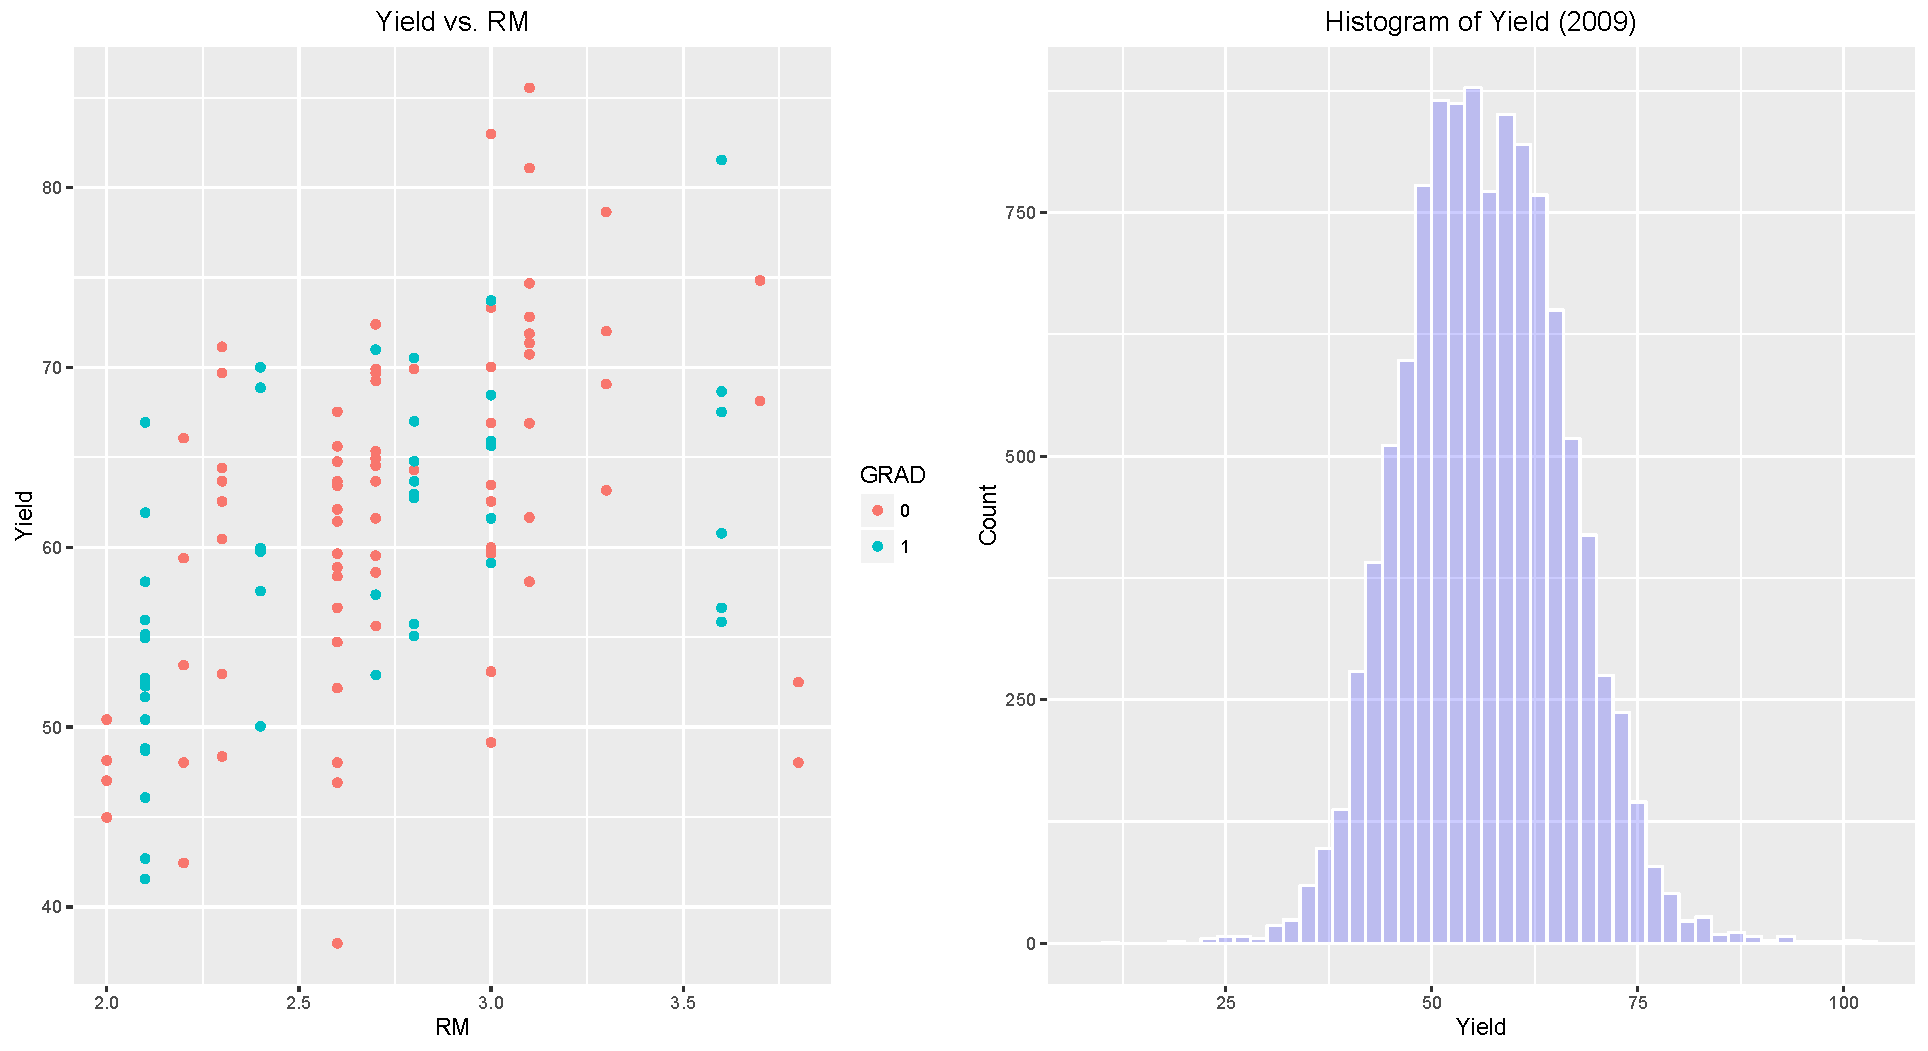
\includegraphics[height = 7cm, width = 12.5cm]{plot1.pdf}
\end{center}
\begin{center}
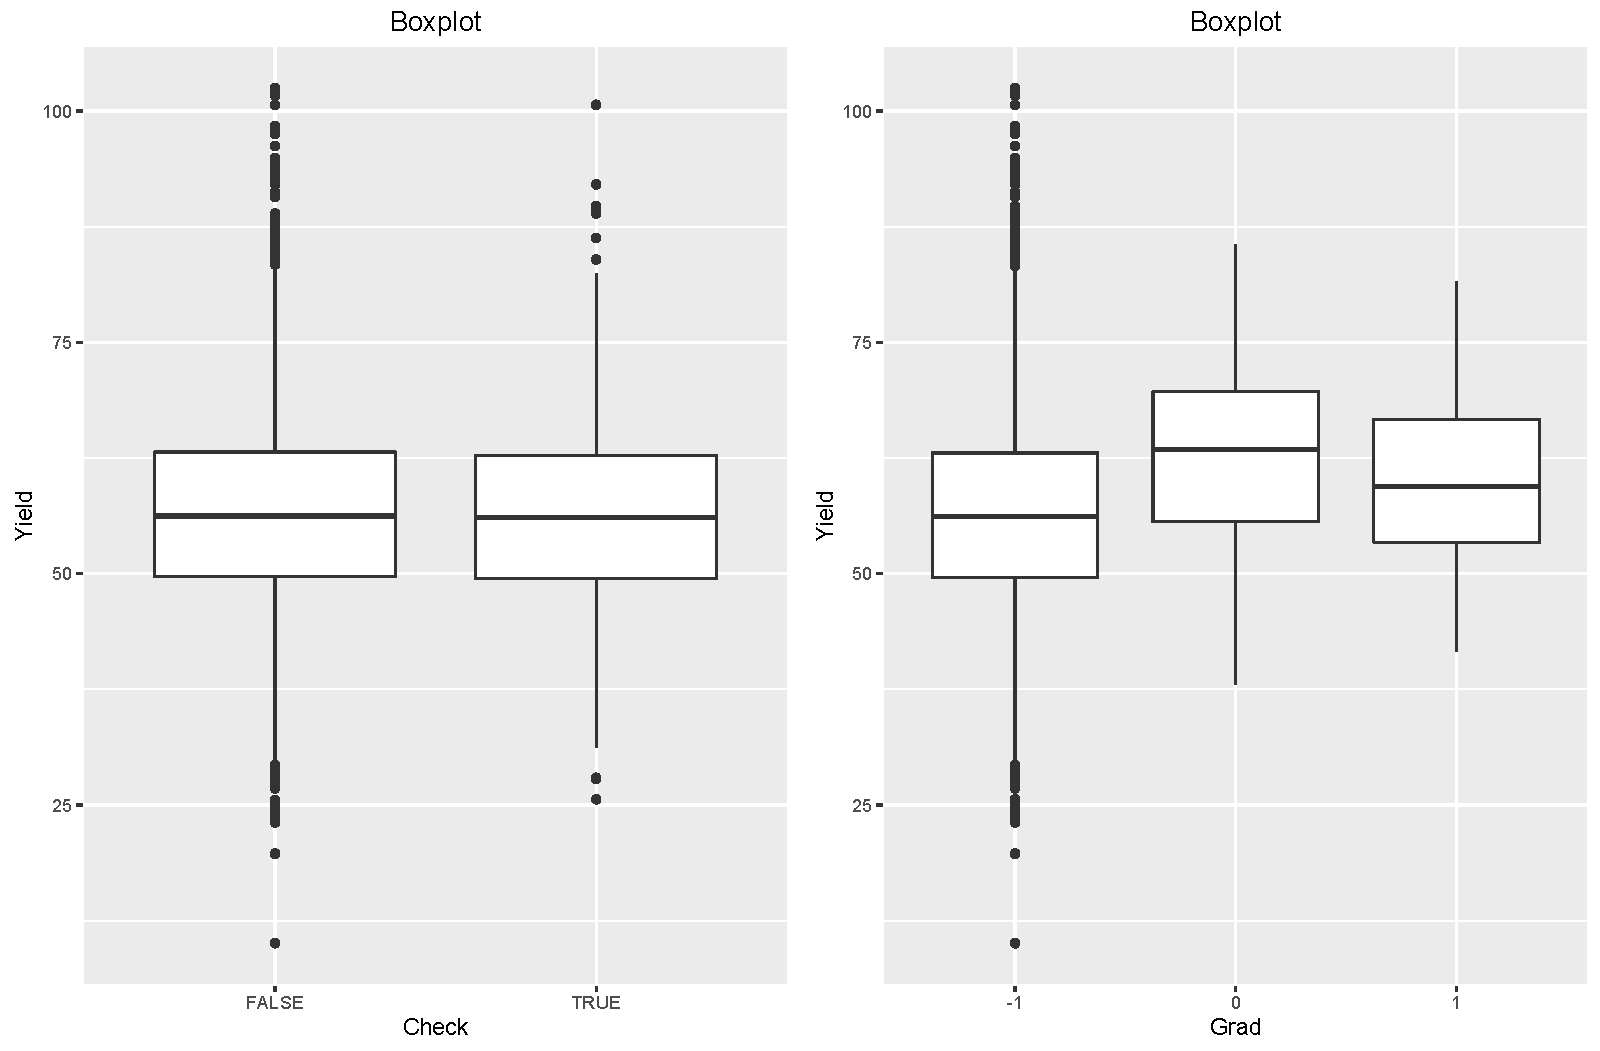
\includegraphics[height = 7cm, width = 12cm]{boxplot.pdf}
\end{center}

\subsection*{Choice of Language and Possible Methodology}
\hfill \\

We will be conducting our analysis mainly in $R$, though we may use some other scripting languages, such as Python and Julia, to automate the I/O and data cleaning beforehand.\\
\\
Even though we are to predict the sales volume, we can still do classification beforehand to do a sanity check. This means that we will most likely be using SVMs for classification, as they are a very robust classification methods.\\
\\
As for now, we are still unsure about what feature transformations or kernels we will be choosing for fitting the data to a linear model, but further investigations later on should give us a better understanding on this issue.



\end{document}